\section{Introduction}

\begin{center}
\makeatletter\def\@captype{figure}\makeatother
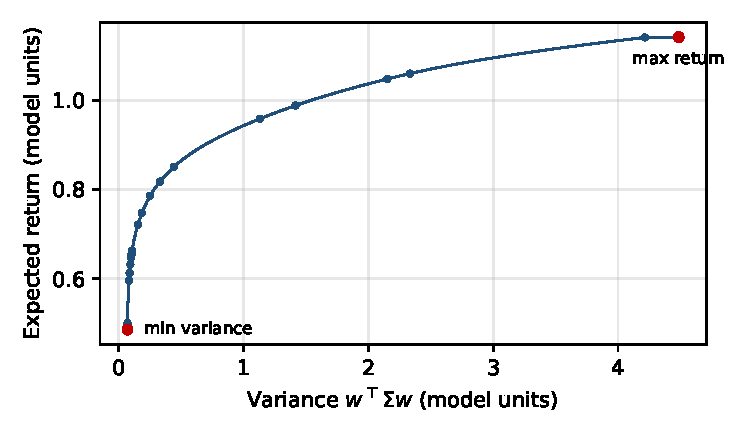
\includegraphics[width=0.65\textwidth]{frontier.pdf}
\caption{The efficient frontier of a $20$-asset long-only problem, traced exactly by
\pkg{cvxcla} as $20$ turning points, plotted as return against variance (\target{frontier}).}
\label{fig:frontier}
\end{center}

The mean--variance portfolio selection problem \citep{markowitz1952} asks for the
allocation of capital across $n$ assets that minimises risk for a given level of
expected return; sweeping the return level produces a one-parameter family of optimal
portfolios whose risk--return image is the \emph{efficient frontier}. The Critical Line
Algorithm (CLA) of \citet{markowitz1956, markowitz1959} represents this frontier
\emph{exactly and in full}: it returns a finite list of \emph{turning points} between
which the frontier is described in closed form, so no discretisation or repeated
re-optimisation is required. The canonical description and a reference implementation
are due to \citet{markowitz2000}; \citet{perold1984}, \citet{stein2008}, and
\citet{hirschberger2010} develop large-scale and active-set variants,
\citet{niedermayer2010} a careful fast implementation, \citet{bailey2013} a widely used
open-source one, and \citet{markowitz2021} a recent review extending the method to
mean--semivariance. In optimisation terms the CLA solves a parametric quadratic
program. \citet{wolfe1959} adapted the simplex method to quadratic programs,
\citet{best1996} gave a parametric active-set algorithm that \citet{best2010} applies to
portfolios, and \pkg{qpOASES} \citep{ferreau2014} is a general parametric QP solver.

Classical CLA implementations take the covariance as a dense matrix. For a large
universe it usually has more structure than that: multi-factor risk models, which
generalise the single-index model \citep{sharpe1963}, write it as a diagonal matrix
plus a low-rank term. The large-scale methods cited above exploit structure through
incremental factorisations, sparsity, or pivoting tied to an explicit matrix.
\pkg{cvxcla} computes the same turning points as any CLA; its contribution is an
\emph{interface} that makes the loop independent of how the covariance is stored, so
the structure becomes a property of an exchangeable backend
(Appendix~\ref{sec:baileydetail}). The mathematics connecting the CLA to the
constrained LASSO, and its history, are the subject of a companion paper
\citep{schmelzer2026perspective}, and \citet{schmelzer2026lasso} shows how to obtain the
efficient frontier from a LASSO solver; this paper documents the software.

\paragraph{Contributions.}
\begin{enumerate}\setlength{\itemsep}{2pt}
\item \textbf{An operator interface.} The turning-point loop reaches the covariance
through a five-member protocol (\S\ref{sec:operators}). A diagonal-plus-low-rank
backend solves the free block through the Woodbury identity, never forms an
$n\times n$ matrix, and traces the same turning points about $40\times$ faster than the dense
backend at $n=2560$, in under $1$~MiB of working memory against $100$~MiB
(\S\ref{sec:experiment}).
\item \textbf{General linear constraints.} Box bounds combine with any linear
equalities $A w = b$ and inequalities $G w \le h$ (\S\ref{sec:ineq}) and a
gross-exposure cap $\lVert w\rVert_1 \le c$ (\S\ref{sec:leverage}).
\item \textbf{A tested implementation.} A least-index tie-break makes the trace
deterministic and provably finite under standard assumptions (\S\ref{sec:bland}); an
independent KKT certificate validates every trace (\S\ref{sec:exactness}); inputs
outside the supported domain are declined with an error that names the cause
(\S\ref{sec:errors}); and one script regenerates every figure and number.
\end{enumerate}
Table~\ref{tab:compare} sets these capabilities against the software a user would
otherwise reach for.

\begin{table}[t]
\centering
\small
\setlength{\tabcolsep}{4pt}
\renewcommand{\arraystretch}{1.5}
\newcolumntype{L}[1]{>{\raggedright\arraybackslash}p{#1}}
\begin{tabular}{L{0.21\textwidth}L{0.20\textwidth}L{0.15\textwidth}L{0.18\textwidth}L{0.13\textwidth}}
\hline
Software & Output & Covariance & Constraints & Gross cap \\
\hline
\pkg{PyPortfolioOpt} \code{CLA} & turning points, some lost & dense matrix & box bounds, one budget row & no \\
QP over a $\lambda$ grid & one portfolio per grid point & as the solver accepts it & any convex & reformulated \\
\pkg{qpOASES} via \pkg{CasADi} & path followed, endpoint returned & matrix & general linear & reformulated \\
\pkg{cvxcla} & every turning point & any operator & box bounds, $Aw=b$, $Gw\le h$ & native lift \\
\hline
\end{tabular}
\caption{What each route to the mean--variance frontier delivers, as used in
\S\ref{sec:experiment}: the QP over a $\lambda$ grid is described in \S\ref{sec:clarabel},
\pkg{qpOASES} in \S\ref{sec:qpoases}, \pkg{cvxcla}'s covariance operators in
\S\ref{sec:operators} and its lift of the gross cap in \S\ref{sec:leverage}. ``Gross
cap'' is $\lVert w\rVert_1 \le c$. ``Path followed, endpoint returned'' means
\pkg{qpOASES} passes the same turning points but does not expose them through
\pkg{CasADi}. The termination
guarantee (\S\ref{sec:bland}) and the KKT certificate (\S\ref{sec:exactness}) are
properties of \pkg{cvxcla}'s trace and are not compared here.}
\label{tab:compare}
\end{table}

We do \emph{not} claim the fastest solve: on small problems \pkg{qpOASES} is faster
(\S\ref{sec:qpoases}), and large dense problems admit faster incremental
factorisations (\S\ref{sec:baseline}).

The package \citep{cvxcla}\footnote{\href{\repourl}{\texttt{github.com/cvxgrp/cvxcla}}}
is built around the class \code{CLA} in \srcfile{src/cvxcla/cla.py}{src/cvxcla/cla.py},
supported by \srcfile{src/cvxcla/first.py}{first.py} (the starting portfolio),
\srcfile{src/cvxcla/operators/__init__.py}{operators/} (the covariance backends), and
\srcfile{src/cvxcla/types.py}{types.py} (the turning-point and frontier data
structures). The notation follows the code.

Sections~\ref{sec:problem}--\ref{sec:iteration} describe the algorithm,
\S\ref{sec:operators} the operator interface, \S\ref{sec:usage} the user interface and
\S\ref{sec:experiment} the experiments; details and the termination proof are in the
appendices.
